
\paragraph{Semaforo privo di enable}
Per la realizzazione una FSM che alterni gli stati come in \figurename{\ref{fig:stati}}
Avendo tre stati diversi è stato necessario impiegare una codifica a 2 bit.
Essendo la codifica arbitraria si riporta la codifica impiegata in 
\tablename{\ref{tab:cod}}.
Essendo possibile con due bit ottenere anche lo stato $00$,  non corrispondente a nessuno degli stati codificati,
è stato imposto che dallo stato $01$ sul successivo fronte di salita di clock il segnale costituisca
la transizione \\VERDE E GIALLO $(0;1)$  $\longrightarrow$ ROSSO $(1;0)$.
Rendendo pertanto il lo stato $0;0$ inaccessibile.
Si riporta la \tablename{ \ref{tab:tran}} delle transizioni tra i vari stati della FSM.
Per la progettazione della macchina è stata impiegata la codifica di Mealy così da minimizzare il numero di porte logiche impiegate.
Dalla \tablename{ \ref{tab:tran}} si ottiene  $b_{1}^{n+1} =  \overline{b_{1}^{n} \cdot b_{0}^{n}}$ e $b_{0}^{n+1} = b_{1}^{n}$

Per realizzare la FSM basata sugli integrati a disposizione, e che realizzi quanto appena descritto,
 è stato realizzato il circuito in \figurename{ \ref{fig:sem2}} alimentando la componentistica con una tensione 
 $V_{cc}\sim 5$\si{\volt}.Si segnala inoltre che in serie con i led sono state montate delle resistenze $R\sim 330$\si{\ohm} per limitare la richiesta di corrente dei diodi LED.
\begin{figure}[h!]
	\begin{minipage}{0.5\textwidth}
		\centering
		\includegraphics[scale=0.20]{immagine.png}
		\caption{Stati della FSM semaforo senza En.}
		\label{fig:stati}
	\end{minipage}
\begin{minipage}{0.5\textwidth}
	\centering
	\begin{tabular}{ssc}
	\toprule
	b_{0} & b_{1} & stato corrispondente\\
	\midrule
	1 & 1 & VERDE\\
	0 & 1 & GIALLO \& VERDE\\
	1 & 0 & ROSSO\\
	0 & 0 &  X (NON VOLUTO)\\
	\bottomrule
	\end{tabular}
	\caption{Codifica degli stati impiegati}
	\label{tab:cod}
\end{minipage}
\end{figure}


\begin{table}[h]
\centering
\begin{tabular}{ss|ss|sss}
	\toprule
	b_{1}^{n} & b_{0}^{n}  & b_{1}^{n+1} & b_{0}^{n+1} & \text{LED VERDE} & \text{LED GIALLO} & \text{LED ROSSO} \\
	\midrule
	 0 & 0 & 0 & 1  & x  & x & x \\
	 0 & 1 & 1 & 1  & 0 & 0 & 1  \\
	 1 & 1 & 1 & 0  & 1 & 0 & 0 \\
	 1 & 0 & 0 & 1  & 1 & 1 & 0 \\
	\bottomrule
\end{tabular}
\caption{Tabella delle transizioni della FSM semaforo sempre abilitato.
Il segnale $1$ corrisponde al LED acceso, $0$ LED spento.
Lo stato $b_{1}=0$ $b_{0}=0$ deve risultare inaccessibile. }
\label{tab:tran}
\end{table}

\begin{figure}[h!]
		\centering
		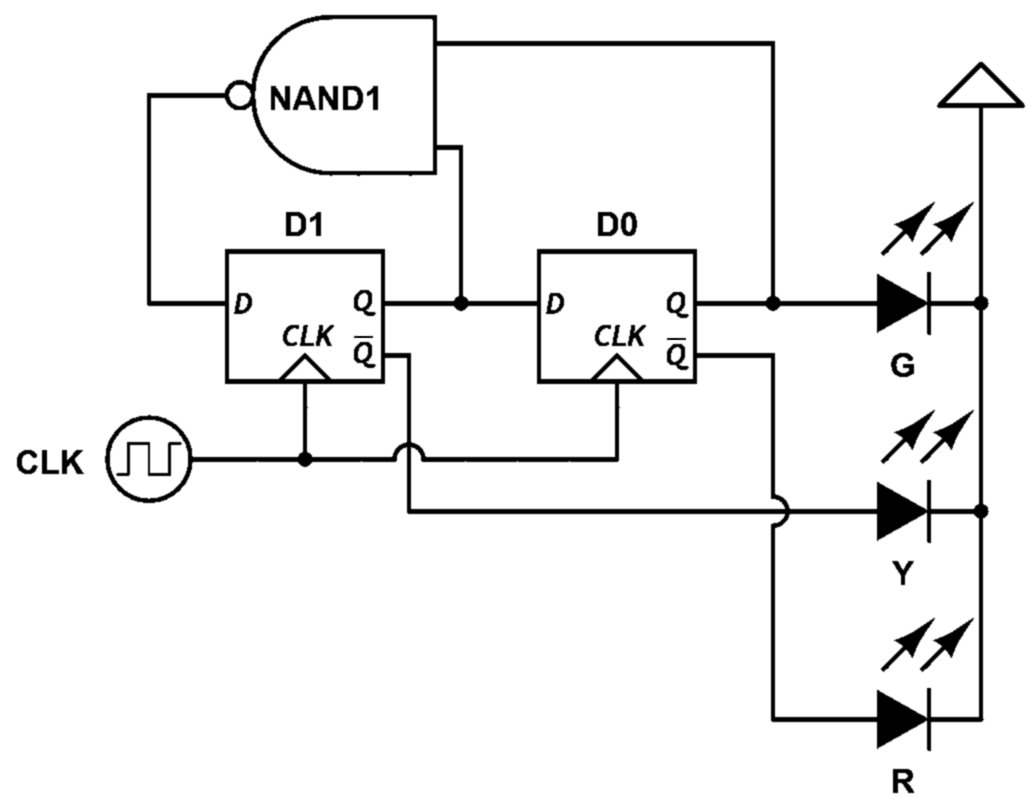
\includegraphics[scale=0.3]{circ3_.png}
		\caption{Circuito che realizzi il semaforo senza En.}
		\label{fig:sem2}
	\end{figure}

Per la verifica del funzionamento circuitale è stato 
 inviato un segnale di clock di frequenza bassa, $f<10 $\si{\hertz} e effettuando un primo controllo attraverso l'accensione dei LED. Si è successivamente aumentata la frequenza di clock $f= $\SI{175.937\pm 0.001}{\hertz}\footnote{Tale misura è stata presa con la funzione di acqusizione automatica dell'oscilloscopio;  l'incertezza associata è la prima cifra che risulti instabile.}
 ed acquisito i valori di tensione corrispondente alle uscite dei vari LED, riportate in 
 \figurename{ \ref{fig:acq}}. Dall'osservazione di
  tali acquisizioni si verifica l'accordo con le specifiche attese. 
 
\begin{figure}[h]
	\centering
	\subfloat[clock ch.1  LED VERDE ch. 2]{
		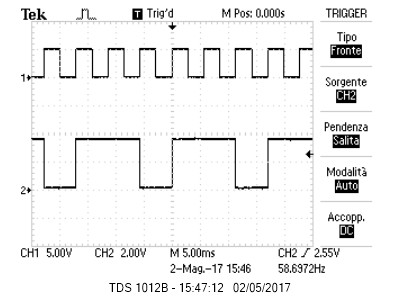
\includegraphics[scale=0.3]{./semaforosemplice/verde.jpg}
	}
	\subfloat[clock ch.1 LED GIALLO ch.2]{
		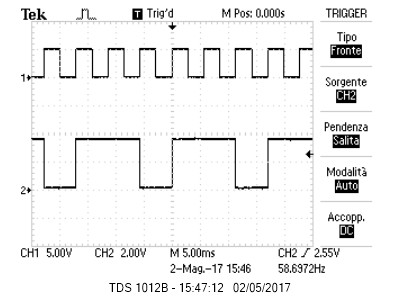
\includegraphics[scale=0.3]{./semaforosemplice/giallo.jpg}
		}\\
	\subfloat[clock ch.1  LED ROSSO ch.2]{
		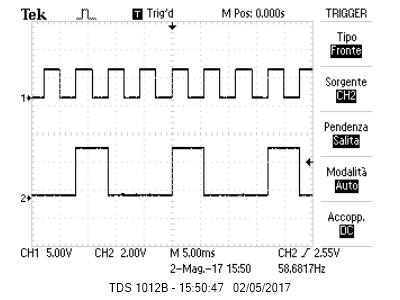
\includegraphics[scale=0.3]{./semaforosemplice/rosso.jpg}
		}
	\subfloat[clock ch.1  $b_{0}$ ch.2]{
		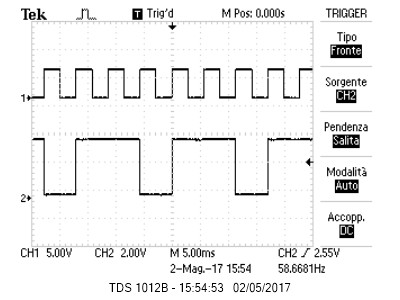
\includegraphics[scale=0.3]{./semaforosemplice/q-.jpg}
		}\\
	\subfloat[clock ch.1 $b_{1}$  ch.2]{
		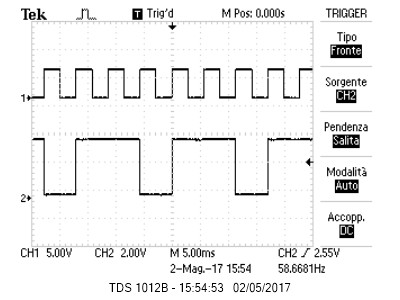
\includegraphics[scale=0.3]{./semaforosemplice/q+.jpg}
	}

	\subfloat[verde ch.1, giallo  ch.2]{
		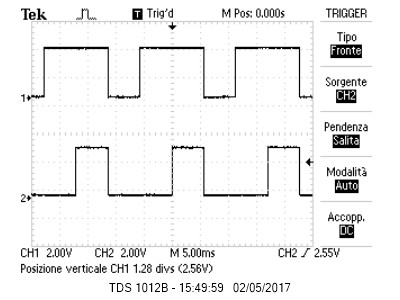
\includegraphics[scale=0.3]{./semaforosemplice/verde_giallo.jpg}
	}
	\subfloat[verde ch.1, rosso  ch.2]{
		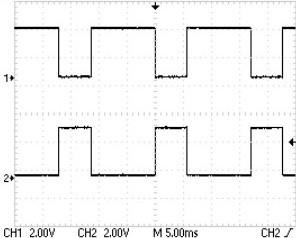
\includegraphics[scale=0.3]{./semaforosemplice/verde_rosso.jpg}
	}
\caption{Acquisizione telle tensioni osservate nel semaforo privo di ENABLE}
\label{fig:acq}
\end{figure}
\paragraph{Semaforo completo}
Per la realizzazione del semaforo completo si è proceduto ad implementare un ulteriore ingresso (En). Tale ingresso svolge la funzione di abilitare il circuito realizzato; in modalità abilitato il circuito realizzare deve comportare come descritto 
nella precedente sezione, mentre qualora si abbia il semaforo disabilitato devono alternarsi gli stati \\TUTTI LED SPENTI $\rightarrow$ LED GIALLO ACCESO ciclicamente.
Essendo arbitraria la codifica del valore di abilitazione è stato imposto che il semaforo sia abilitato
per $En = 1$; si è optato inoltre per realizzare un segnale di ENABLE sincrono; pertanto è stato aggiunto rispetto al 
circuito precedente un ulteriore FLIP-FLOP D-LEATCH.

Si riporta la  tabella di verita in \tablename{\ref{tab:tran2}}


\begin{table}[h]
	\centering
	\begin{tabular}{sss|ss|sss}
		\toprule
		b_{1}^{n} & b_{0}^{n} & En  & b_{1}^{n+1} & b_{0}^{n+1} & \text{LED VERDE} & \text{LED GIALLO} & \text{LED ROSSO} \\
		\midrule
		0 & 0 & 0& x & x & x & x& x\\
		0 & 0 & 1& 1 & 0 &  & & \\
		0 & 1 & 0& 1 & 1 &  & & \\
		0 & 1 & 1& 1 & 0 &  & & \\
		1 & 0 & 0& x & x &  & & \\
		1 & 0 & 1& 1 & 1 &  & & \\
		1 & 1 & 0& 0 & 1 &  & & \\
		1 & 1 & 1& 0 & 1 &  & & \\
		\bottomrule
	\end{tabular}
	\caption{Tabella delle transizioni della FSM semaforo completo.
		Il segnale $1$ corrisponde al LED acceso, $0$ LED spento.CONTROLLARE }
	\label{tab:tran2}
\end{table}
